\section{Geomagnetic Field -- IGRF}
Although the broad properties of the Geomagnetic field have been known for centuries, the first systematic study of the field was begun in the early nineteenth century by German mathematician and physicist Gauss as found in Wertz \cite{wertz2012spacecraft}. Jeffrey \cite{love2008magnetic} stating that around 170 observatories networks around the globe are used to report geomagnetic data. Throughout 120 observatories now produce and frequently report digital data with a one-minute collection cadence or better; figure \ref{fig:obs} below depicts their locations around the world. The remaining 50 or so observatories rely on outdated, analogue equipment or provide data years after it has been collected.

\begin{figure}[H]
    \centering
    \includegraphics[width = \textwidth]{Figures/obseratories.jpg}
    \caption{Worldwide Distribution of Geomagnetic Observatories}
    \label{fig:obs}
\end{figure}


Wertz \cite{wertz2012spacecraft} elaborated that despite the fact that this collection of data has improved our capacity to precisely characterise the field, it still lacks the key to the physical processes that make or disturb it. As a result, we shall discuss the observed occurrences in this part and, when feasible, present compelling justifications for their existence.


\subsection{Geomagnetic Field Definition}
The geomagnetic field is primarily that of a magnetic dipole, like that produced by a sphere of uniform magnetization or a current loop. In 1975, the dipole's strength was $7.96 \times 10^{15}$ Wb.m. The dipole's "south" end was located at 78.60° N latitude and 289.55° E longitude in the northern hemisphere, migrating westward at a rate of around 0.014 degrees each year. The dipole strength is dropping at a rate of 0.05 percent every year.

The magnetic equator is the plane perpendicular to the Earth-centered dipole. The field is weakest there, with a strength of around $3\times10^4$ nT near the Earth's surface. At the magnetic equator, figure \ref{fig:alt} below depicts the fluctuation in dipole field intensity as a function of height \cite{wertz2012spacecraft}.

As the magnetic latitude increases from 0 to 90 degrees, the field strength increases by a factor of two, as seen in figure \ref{fig:lat}. The field is horizontal relative to the Earth's surface at the geomagnetic equator. The field is 45 degrees down from horizontal at a geomagnetic latitude of around 27 degrees \cite{wertz2012spacecraft}.

\begin{figure}[H]
     \centering
     \begin{subfigure}[b]{0.45\textwidth}
         \centering
          \includegraphics[width =\textwidth]{Figures/alt.png}   
          \subcaption{Fluctuation in dipole field intensity as a function of height.}
               \label{fig:alt}
          \end{subfigure}
     \hfill
     \begin{subfigure}[b]{0.48\textwidth}
         \centering
         \includegraphics[width=\textwidth, angle = 90]{Figures/lat.png}
         \subcaption{Field strength as function of magnetic latitude.}
              \label{fig:lat}
     \end{subfigure}
     \caption{Magnetic intensity as function of altitude and latitude.}

\end{figure}

\subsection{Mathematical Model}
\label{sec:igrf_math}
The International Geomagnetic Reference Field (IGRF) is a set of spherical harmonic coefficients that may be entered into a mathematical model to explain the big, time-varying component of the Earth's core magnetic field between 1900 A.D. and the present. Under the auspices of the Multinational Association of Geomagnetism and Aeronomy (IAGA) Working Group V-MOD, an international task force of scientists creates and maintains the IGRF \cite{alken2021international}.

The IGRF defines the primary geomagnetic field $B(x,y,z,t)$ created by internal sources largely within the Earth's core. The IGRF is valid on and above the Earth's surface, where the primary geomagnetic field may be characterised by the following equation.
\begin{equation}
    \label{eqn:IGRF1}
    \mathbf{B}_{\lambda}(x, y, z, t) = - R_{\oplus}^2 \times Real \left\{\sum_{n=1}^{\infty} \sum_{m=0}^{n} R_{\oplus}^n (g_n^m -  h_n^m i) \frac{\partial V_{n,m}}{\partial \lambda}  d_{n,m} \right\}
\end{equation}
Where,
\begin{gather*} 
\lambda = x, y, z.\\
i =\sqrt{-1}.\\
R_{\oplus}\triangleq \text{Earth’s radius}.\\
g_n, \, h_n \triangleq \text{The Gaussian magnetic field coefficients}.
\end{gather*}
The values for $d_{n,m}$ and $V_{n,m}$ can be calculated as following.
\begin{gather} 
d_{1,0} = 1, \; d_{1,1} = 1, \; d_{0,0} = 1 \\
d_{n,n} = \frac{d_{n-1,n-1}}{\sqrt{(2n-1)\times2n}}\\
d_{n,m} = \sqrt{2 \times \frac{(n-m)!}{(n+m)!}}\\
V_{n,n} = (2n - 1) \times \frac{(x+iy)\times V_{n-1,n-1}}{r^2}\\
V_{n,m} = \begin{dcases}
 \frac{(2n-1)\times z \times V_{n-1,m}}{(n-m)\times r^2}, &\mbox{if } n-m = 1 \\
 \frac{(2n-1) \times z \times V_{n-1,m}}{(n-m)\times r^2} - \frac{(n+m-1)\times  V_{n-2,m}}{(n-m) \times r^2}, &\mbox{if } n-m > 1
\end{dcases}
\end{gather}
\begin{gather}
    \frac{\partial V_{n,m}}{\partial x} = \begin{dcases}
    - \frac{1}{2} \times \left(V_{n+1,m} + \overline{V}_{n+1,1} \right) , &\mbox{if } m = 0 \\
    -\frac{1}{2} \times \left(V_{n+1,m+1} - \frac{(n-m+2)!}{(n-m)!} V_{n+1,m-1} \right), &\mbox{if } m > 1
\end{dcases}
\end{gather}
\begin{gather}
   \frac{\partial V_{n,m}}{\partial y} = \begin{dcases}
    - \frac{i}{2} \times \left(V_{n+1,m} - \overline{V}_{n+1,1} \right) , &\mbox{if } m = 0 \\
    -\frac{i}{2} \times \left(V_{n+1,m+1} + \frac{(n-m+2)!}{(n-m)!} V_{n+1,m-1} \right), &\mbox{if } m > 1
\end{dcases}
\end{gather}
\begin{gather}
    \frac{\partial V_{n,m}}{\partial z} = \frac{(n-m+1)!}{(n-m)!} V_{n+1,m}
\end{gather}
Where the complex-conjugate value of function $V_{n+1,1}$ is denoted as $\overline{V}_{n+1,1}$.

The values of the coefficients gn,m and hn,m of the first harmonic up to 13 orders inclusive, are retrieved from the International Geomagnetic Reference Field 13th edition \cite{alken2021international}. Using the coefficients presented in the IGRF 13th edition, the upcoming coefficients for the consecutive years can be calculated using the secular variation by the following equations.
\begin{equation}
    g_n^m(t) = g_n^m(T_t) + (t-T_t)\dot{g}_n^m(T_t)
\end{equation}
\begin{equation}
        h_n^m(t) = h_n^m(T_t) + (t-T_t)\dot{h}_n^m(T_t)
\end{equation}
Where $g_n^m(T_t)$ and $h_n^m (T_t)$ are the Gauss coefficients at the time t preceding epoch $T_t$. The model epochs in IGRF-13 are given in precise multiples of 5 years beginning in 1900 and ending in 2020 (see Table \ref{tab:g_nm} and \ref{tab:h_nm} for 2020 values), hence $T_t \leqslant t < T_t + 5$. The specifications for $T_t < 2020$.


\begin{table}[H]
\centering
\resizebox{\textwidth}{!}{%
\begin{tabular}{@{}lrrrrrrrrrrrrrr@{}}
\toprule
$n/m$                   & 1        & 2       & 3      & 4      & 5      & 6     & 7     & 8     & 9    & 10    & 11   & 12   & 13   & 14   \\ \midrule
\multicolumn{1}{l|}{1}  & 0        & 0       & 0      & 0      & 0      & 0     & 0     & 0     & 0    & 0     & 0    & 0    & 0    & 0    \\
\multicolumn{1}{l|}{2}  & -29404.8 & -1450.9 & 0      & 0      & 0      & 0     & 0     & 0     & 0    & 0     & 0    & 0    & 0    & 0    \\
\multicolumn{1}{l|}{2}  & -2499.6  & 2982.0  & 1677.0 & 0      & 0      & 0     & 0     & 0     & 0    & 0     & 0    & 0    & 0    & 0    \\
\multicolumn{1}{l|}{3}  & 1363.2   & -2381.2 & 1236.2 & 525.7  & 0      & 0     & 0     & 0     & 0    & 0     & 0    & 0    & 0    & 0    \\
\multicolumn{1}{l|}{4}  & 903.0    & 809.5   & 86.3   & -309.4 & 48.0   & 0     & 0     & 0     & 0    & 0     & 0    & 0    & 0    & 0    \\
\multicolumn{1}{l|}{5}  & -234.3   & 363.2   & 187.8  & -140.7 & -151.2 & 13.5  & 0     & 0     & 0    & 0     & 0    & 0    & 0    & 0    \\
\multicolumn{1}{l|}{6}  & 66.0     & 65.5    & 72.9   & -121.5 & -36.2  & 13.5  & -64.7 & 0     & 0    & 0     & 0    & 0    & 0    & 0    \\
\multicolumn{1}{l|}{7}  & 80.6     & -76.7   & -8.2   & 56.5   & 15.8   & 6.4   & -7.2  & 9.8   & 0    & 0     & 0    & 0    & 0    & 0    \\
\multicolumn{1}{l|}{8}  & 23.7     & 9.7     & -17.6  & -0.5   & -21.1  & 15.3  & 13.7  & -16.5 & -0.3 & 0     & 0    & 0    & 0    & 0    \\
\multicolumn{1}{l|}{9}  & 5.0      & 8.4     & 2.9    & -1.5   & -1.1   & -13.2 & 1.1   & 8.8   & -9.3 & -11.9 & 0    & 0    & 0    & 0    \\
\multicolumn{1}{l|}{10} & -1.9     & -6.2    & -0.1   & 1.7    & -0.9   & 0.7   & -0.9  & 1.9   & 1.4  & -2.4  & -3.8 & 0    & 0    & 0    \\
\multicolumn{1}{l|}{11} & 3.0      & -1.4    & -2.5   & 2.3    & -0.9   & 0.3   & -0.7  & -0.1  & 1.4  & -0.6  & 0.2  & 3.1  & 0    & 0    \\
\multicolumn{1}{l|}{12} & -2.0     & -0.1    & -0.1   & 1.3    & -1.2   & 0.7   & 0.3   & 0.5   & -0.3 & -0.5  & 0.1  & -1.1 & -0.3 & 0    \\
\multicolumn{1}{l|}{13} & 0.1      & -0.9    & 0.5    & 0.7    & -0.3   & 0.8   & 0.0   & 0.8   & 0.0  & 0.4   & 0.1  & 0.5  & -0.5 & -0.4 \\ \bottomrule
\end{tabular}%
}
\caption{$g_n^m$ Values as provided in IGRF-13 Generation}
\label{tab:g_nm}
\end{table}


\begin{table}[H]
\centering
\resizebox{\textwidth}{!}{%
\begin{tabular}{@{}lrrrrrrrrrrrrrr@{}}
\toprule
                        & 1 & 2       & 3      & 4      & 5      & 6    & 7     & 8    & 9    & 10   & 11   & 12   & 13   & 14   \\ \midrule
\multicolumn{1}{l|}{1}  & 0 & 0       & 0      & 0      & 0      & 0    & 0     & 0    & 0    & 0    & 0    & 0    & 0    & 0    \\
\multicolumn{1}{l|}{2}  & 0 & 4652.5  & 0      & 0      & 0      & 0    & 0     & 0    & 0    & 0    & 0    & 0    & 0    & 0    \\
\multicolumn{1}{l|}{2}  & 0 & -2991.6 & -734.6 & 0      & 0      & 0    & 0     & 0    & 0    & 0    & 0    & 0    & 0    & 0    \\
\multicolumn{1}{l|}{3}  & 0 & -82.1   & 241.9  & -543.4 & 0      & 0    & 0     & 0    & 0    & 0    & 0    & 0    & 0    & 0    \\
\multicolumn{1}{l|}{4}  & 0 & 281.9   & -158.4 & 199.7  & -349.7 & 0    & 0     & 0    & 0    & 0    & 0    & 0    & 0    & 0    \\
\multicolumn{1}{l|}{5}  & 0 & 47.7    & 208.3  & -121.2 & 32.3   & 98.9 & 0     & 0    & 0    & 0    & 0    & 0    & 0    & 0    \\
\multicolumn{1}{l|}{6}  & 0 & -19.1   & 25.1   & 52.8   & -64.5  & 8.9  & 68.1  & 0    & 0    & 0    & 0    & 0    & 0    & 0    \\
\multicolumn{1}{l|}{7}  & 0 & -51.5   & -16.9  & 2.2    & 23.5   & -2.2 & -27.2 & -1.8 & 0    & 0    & 0    & 0    & 0    & 0    \\
\multicolumn{1}{l|}{8}  & 0 & 8.4     & -15.3  & 12.8   & -11.7  & 14.9 & 3.6   & -6.9 & 2.8  & 0    & 0    & 0    & 0    & 0    \\
\multicolumn{1}{l|}{9}  & 0 & -23.4   & 11     & 9.8    & -5.1   & -6.3 & 7.8   & 0.4  & -1.4 & 9.6  & 0    & 0    & 0    & 0    \\
\multicolumn{1}{l|}{10} & 0 & 3.4     & -0.2   & 3.6    & 4.8    & -8.6 & -0.1  & -4.3 & -3.4 & -0.1 & -8.8 & 0    & 0    & 0    \\
\multicolumn{1}{l|}{11} & 0 & 0       & 2.5    & -0.6   & -0.4   & 0.6  & -0.2  & -1.7 & -1.6 & -3   & -2   & -2.6 & 0    & 0    \\
\multicolumn{1}{l|}{12} & 0 & -1.2    & 0.5    & 1.4    & -1.8   & 0.1  & 0.8   & -0.2 & 0.6  & 0.2  & -0.9 & 0    & 0.5  & 0    \\
\multicolumn{1}{l|}{13} & 0 & -0.9    & 0.6    & 1.4    & -0.4   & -1.3 & -0.1  & 0.3  & -0.1 & 0.5  & 0.5  & -0.4 & -0.4 & -0.6 \\ \bottomrule
\end{tabular}%
}
\caption{$h_n^m$ Values as provided in IGRF-13 Generation}
\label{tab:h_nm}
\end{table}

\subsection{MATLAB Model Implementation}

\subsubsection{calculate\_d\_nm.m}
MATLAB-function to compute the value of $d_{n,m}$. The function takes no input and the output is described in table \ref{tab:d}.
\begin{table}[H]
\centering
\caption{IN/OUT parameters of calculate\_d\_nm.m}
\label{tab:d}
\begin{tabular}{lll}
\rowcolor[HTML]{000000} 
\multicolumn{3}{l}{\cellcolor[HTML]{000000}{\color[HTML]{FFFFFF} calculate\_d\_nm.m: calculates the value of $d_{n,m}$ function}}                                                \\
\rowcolor[HTML]{000000} 
{\color[HTML]{FFFFFF} \textbf{IN/OUT}} & {\color[HTML]{FFFFFF} \textbf{Var. Name}} & {\color[HTML]{FFFFFF} \textbf{Description}} \\
OUT & d\_nm & 14-by-14 matrix storing the values of d\_nm

\end{tabular}%
\end{table}


\subsubsection{calculate\_v.m}
MATLAB-function to compute the value of $V$. The IN/OUT parameters are described in table \ref{tab:v}.
\begin{table}[H]
\centering
\caption{IN/OUT parameters of calculate\_v.m}
\label{tab:v}
\begin{tabular}{lll}
\rowcolor[HTML]{000000} 
\multicolumn{3}{l}{\cellcolor[HTML]{000000}{\color[HTML]{FFFFFF} calculate\_v.m: calculates the value of $d_{n,m}$ function}}                                                \\
\rowcolor[HTML]{000000} 
{\color[HTML]{FFFFFF} \textbf{IN/OUT}} & {\color[HTML]{FFFFFF} \textbf{Var. Name}} & {\color[HTML]{FFFFFF} \textbf{Description}} \\
OUT & v & 14-by-14 matrix storing the values of V\\
IN & x & x coordinate of the point of interest\\
IN & y & y coordinate of the point of interest\\
IN & z & z coordinate of the point of interest
\end{tabular}%
\end{table}

\subsubsection{calc\_partial\_v.m}
MATLAB-function to compute $\partial V / \partial \lambda$. The IN/OUT parameters are described in table \ref{tab:partial_v}.
\begin{table}[H]
\centering
\caption{IN/OUT parameters of calc\_partial\_v.m}
\label{tab:partial_v}
\begin{tabular}{lll}
\rowcolor[HTML]{000000} 
\multicolumn{3}{l}{\cellcolor[HTML]{000000}{\color[HTML]{FFFFFF} calc\_partial\_v.m: calculates the partial derivative of v with respect to x, y, and z.}}                                                \\
\rowcolor[HTML]{000000} 
{\color[HTML]{FFFFFF} \textbf{IN/OUT}} & {\color[HTML]{FFFFFF} \textbf{Var. Name}} & {\color[HTML]{FFFFFF} \textbf{Description}} \\
OUT & partial\_v\_x & the derivative of V with respect to x\\
OUT & partial\_v\_y & the derivative of V with respect to y\\
OUT & partial\_v\_z & the derivative of V with respect to z\\
IN & v & 14-by-14 matrix containing the values of v
\end{tabular}%
\end{table}

\subsubsection{read\_coef.m}
MATLAB-function to read the coefficients of the IGRF model. The function takes no input and the output is described in table \ref{tab:read}.
\begin{table}[H]
\centering
\caption{IN/OUT parameters of read\_coef.m}
\label{tab:read}
\begin{tabular}{lll}
\rowcolor[HTML]{000000} 
\multicolumn{3}{l}{\cellcolor[HTML]{000000}{\color[HTML]{FFFFFF} read\_coef.m: reads the IGRF Coefficients}}                                                \\
\rowcolor[HTML]{000000} 
{\color[HTML]{FFFFFF} \textbf{IN/OUT}} & {\color[HTML]{FFFFFF} \textbf{Var. Name}} & {\color[HTML]{FFFFFF} \textbf{Description}} \\
OUT & g\_nm & the values of $g_{nm}$\\
OUT & h\_nm & the values of $h_{nm}$\\
OUT & g\_nm\_dot & the values of $\dot{g}_{n,m}$\\
OUT & h\_nm\_dot & the values of $\dot{h}_{n,m}$
\end{tabular}%
\end{table}


\subsubsection{magneticFieldModel.m}
MATLAB-function to model the IGRF mathematical representation discussed in section \ref{sec:igrf_math}. It computes the magnetic field components in $x, y, \text{ and}, z$ directions as well as the total magnetic field in ECI. The IN/OUT attributes is described in table \ref{tab:igrf}.
\begin{table}[H]
\centering
\caption{IN/OUT parameters of magneticFieldModel.m}
\label{tab:igrf}
\begin{tabular}{lll}
\rowcolor[HTML]{000000} 
\multicolumn{3}{l}{\cellcolor[HTML]{000000}{\color[HTML]{FFFFFF} magneticFieldModel.m: Modeling the geo-magnetic field}}                                                \\
\rowcolor[HTML]{000000} 
{\color[HTML]{FFFFFF} \textbf{IN/OUT}} & {\color[HTML]{FFFFFF} \textbf{Var. Name}} & {\color[HTML]{FFFFFF} \textbf{Description}} \\
OUT & B\_x & the geomagnetic field component in x direction\\
OUT & B\_y & the geomagnetic field component in y direction\\
OUT & B\_z & the geomagnetic field component in z direction\\
OUT & total & the total geomagnetic field\\
IN & lat & the latitude of the point of interest \\
IN & lon & the longitude of the point of interest \\
IN & lat & the altitude of the point of interest
\end{tabular}%
\end{table}



%%%%%%%%%%%%%%%%%%%%%%%%%%%%%%%%%%%%%%%%%%%%%%%%%%%%%%%%%%%%%%%
\subsection{Results of The MATLAB Model}
A MATLAB code is made for this mathematical model in order to get the earths' magnetic field contours at given altitude and time. 
Figure \ref{fig:res} shows the Total Field at the ellipsoid surface for epoch 2020 at earths' surface.
\begin{figure}[H]
    \centering
    \includegraphics[width = \textwidth]{Figures/total_mag_field_2020.png}
    \caption{Total Geomagnetic Field contours in nT as depicted by MATLAB simulation.}
    \label{fig:res}
\end{figure}

\section{Geo-Gravitational Field -- Spherical Harmonics Gravity}
\subsection{Definition}
Two point masses, $M$ and $m$, separated by a vector distance $r$, are attracted to one other by a force described by Newton's law of gravity
\begin{equation}
    F=G \frac{M m}{r^{2}} \bar{r}
\end{equation}
If $M_{\oplus}$ is the mass of the Earth and $m$ is the mass of the body whose motion we wish to follow, then it is convenient to define the geocentric gravitational constant, $\mu_{\oplus}$, and the Earth gravitational potential, $\boldsymbol{U}$ by
\begin{equation*}
\begin{gathered}
\mu_{\oplus}=G M_{\oplus} \\
\boldsymbol{U}=-\frac{G M_{\oplus}}{r}, \\
\end{gathered}
\end{equation*}
The force equation becomes
\begin{equation}
    \boldsymbol{F}=-\frac{\mu_{\oplus} m}{r^{2}}\bar{\boldsymbol{r}}=-m \nabla \boldsymbol{U}
\end{equation}
\subsection{Mathematical Model}
For this Model a MATLAB code is carried out and can be found in appendix \ref{app:matlab_Gravity}.

\begin{equation}
\frac{\partial U}{\partial \lambda}=\operatorname{real}\left(\sum_{n=1}^{\infty} \sum_{m=0}^{n} R_{e}^{n}\left(C_{n m}-j * S_{n m}\right) * \frac{\partial V_{n, m}}{\partial \lambda}\right)
\end{equation}
Where
\begin{gather*} 
\lambda = x, y, z.\\
i =\sqrt{-1}.\\
R_{\oplus} \triangleq \text{Earth’s radius}.\\
C_{nm}, \, S_{nm} \triangleq \text{The Earth's gravity coefficients}.
\end{gather*}
\begin{equation}
    V_{0,0} = \frac{1}{r}
\end{equation}
\begin{equation}
    V_{n,n} = (2n - 1) \times \frac{(x+iy)\times V_{n-1,n-1}}{r^2}
\end{equation}
\begin{gather} 
V_{n,m} = \begin{dcases}
 \frac{(2n-1)\times z \times V_{n-1,m}}{(n-m)\times r^2}, &\mbox{if } n-m = 1 \\
 \frac{(2n-1) \times z \times V_{n-1,m}}{(n-m)\times r^2} - \frac{(n+m-1)\times  V_{n-2,m}}{(n-m) \times r^2}, &\mbox{if } n-m > 1
\end{dcases}
\end{gather}
\begin{gather}
    \frac{\partial V_{n,m}}{\partial x} = \begin{dcases}
    - \frac{1}{2} \times \left(V_{n+1,m} + \overline{V}_{n+1,1} \right) , &\mbox{if } m = 0 \\
    -\frac{1}{2} \times \left(V_{n+1,m+1} - \frac{(n-m+2)!}{(n-m)!} V_{n+1,m-1} \right), &\mbox{if } m > 1
\end{dcases}
\end{gather}
\begin{gather}
   \frac{\partial V_{n,m}}{\partial x} = \begin{dcases}
    - \frac{i}{2} \times \left(V_{n+1,m} - \overline{V}_{n+1,1} \right) , &\mbox{if } m = 0 \\
    -\frac{i}{2} \times \left(V_{n+1,m+1} + \frac{(n-m+2)!}{(n-m)!} V_{n+1,m-1} \right), &\mbox{if } m > 1
\end{dcases}
\end{gather}
\begin{gather}
    \frac{\partial V_{n,m}}{\partial z} = \frac{(n-m+1)!}{(n-m)!} V_{n+1,m}
\end{gather}
The values of each $C_{nm}$ and $S_{nm}$ are both retrieved from \cite{wertz2012spacecraft}.
The gravity vector will be
\begin{equation}
\boldsymbol{g}=\mu_{\oplus}\left[\begin{array}{l}
\frac{\partial U}{\partial x} \\
\frac{\partial U}{\partial y} \\
\frac{\partial U}{\partial z}
\end{array}\right]
\end{equation}

\subsection{MATLAB Model Implementation}

\subsubsection{calculate\_v.m}
MATLAB-function to compute the value of $V$. The IN/OUT parameters are described in table \ref{tab:v_grav}.
\begin{table}[H]
\centering
\caption{IN/OUT parameters of calc\_v.m}
\label{tab:v_grav}
\begin{tabular}{lll}
\rowcolor[HTML]{000000} 
\multicolumn{3}{l}{\cellcolor[HTML]{000000}{\color[HTML]{FFFFFF} calculate\_v.m: calculates the value of $d_{n,m}$ function}}                                                \\
\rowcolor[HTML]{000000} 
{\color[HTML]{FFFFFF} \textbf{IN/OUT}} & {\color[HTML]{FFFFFF} \textbf{Var. Name}} & {\color[HTML]{FFFFFF} \textbf{Description}} \\
OUT & v & 7-by-7 matrix storing the values of V\\
IN & x & x coordinate of the point of interest\\
IN & y & y coordinate of the point of interest\\
IN & z & z coordinate of the point of interest
\end{tabular}%
\end{table}
\subsubsection{calculate\_partial\_v.m}
MATLAB-function to compute $\partial V / \partial \lambda$. The IN/OUT parameters are described in table \ref{tab:partial_v_grav}.
\begin{table}[H]
\centering
\caption{IN/OUT parameters of calc\_partial\_v.m}
\label{tab:partial_v_grav}
\begin{tabular}{lll}
\rowcolor[HTML]{000000} 
\multicolumn{3}{l}{\cellcolor[HTML]{000000}{\color[HTML]{FFFFFF} calc\_partial\_v.m: calculates the partial derivative of v with respect to x, y, and z.}}                                                \\
\rowcolor[HTML]{000000} 
{\color[HTML]{FFFFFF} \textbf{IN/OUT}} & {\color[HTML]{FFFFFF} \textbf{Var. Name}} & {\color[HTML]{FFFFFF} \textbf{Description}} \\
OUT & partial\_v\_x & the derivative of V with respect to x\\
OUT & partial\_v\_y & the derivative of V with respect to y\\
OUT & partial\_v\_z & the derivative of V with respect to z\\
IN & v & 7-by-7 matrix containing the values of v
\end{tabular}%
\end{table}


\subsubsection{read\_coef.m}
MATLAB-function to read the coefficients of the IGRF model. The function takes no input and the output is described in table \ref{tab:read_grav}.
\begin{table}[H]
\centering
\caption{\textit{MATLAB function} -- reading $g_{n,m}$, $h_{n,m}$, $\dot{g}_{n,m}$, $\dot{h}_{n,m}$}
\label{tab:read_grav}
\begin{tabular}{lll}
\rowcolor[HTML]{000000} 
\multicolumn{3}{l}{\cellcolor[HTML]{000000}{\color[HTML]{FFFFFF} read\_coef.m: reads the IGRF Coefficients}}                                                \\
\rowcolor[HTML]{000000} 
{\color[HTML]{FFFFFF} \textbf{IN/OUT}} & {\color[HTML]{FFFFFF} \textbf{Var. Name}} & {\color[HTML]{FFFFFF} \textbf{Description}} \\
OUT & g\_nm & the values of $g_{nm}$\\
OUT & h\_nm & the values of $h_{nm}$\\
OUT & g\_nm\_dot & the values of $\dot{g}_{n,m}$\\
OUT & h\_nm\_dot & the values of $\dot{h}_{n,m}$
\end{tabular}%
\end{table}

\subsubsection{calculate\_gravity.m}
MATLAB-function to calculate the earth's gravity. It computes the gravity field components in $x, y, \text{ and}, z$ directions as well as the total gravity. The IN/OUT attributes is described in table \ref{tab:grav}.
\begin{table}[H]
\centering
\caption{IN/OUT parameters of calculate\_gravity.m}
\label{tab:grav}
\begin{tabular}{lll}
\rowcolor[HTML]{000000} 
\multicolumn{3}{l}{\cellcolor[HTML]{000000}{\color[HTML]{FFFFFF} calculate\_gravity.m: Modeling the gravity field}}                                                \\
\rowcolor[HTML]{000000} 
{\color[HTML]{FFFFFF} \textbf{IN/OUT}} & {\color[HTML]{FFFFFF} \textbf{Var. Name}} & {\color[HTML]{FFFFFF} \textbf{Description}} \\
OUT & g\_x & the gravity field component in x direction\\
OUT & g\_y & the gravity field component in y direction\\
OUT & g\_z & the gravity field component in z direction\\
OUT & g_tot & the total gravity field\\
IN & x & the x coordinate in ECI of the point of interest \\
IN & y & the y coordinate in ECI of the point of interest\\
IN & z & the z coordinate in ECI of the point of interest
\end{tabular}%
\end{table}



%%%%%%%%%%%%%%%%%%%%%%%%%%%%%%%
\section{Eclipse Time}
\subsection{Definition}
When a satellite orbiting the earth passes into a shadow zone, depriving the solar arrays of sunlight, the time duration for the orbit in this shadow zone change with the variation of the orbit type. This period of time is referred to as eclipse time, and the shadow zone is referred to as eclipse region. In the eclipse time, a secondary power source is used to provide power to the satellite's variant subsystems. Batteries are usually used as this secondary power source. Thus, calculating eclipse time is critical for battery sizing and maintaining a steady heat balance within the satellite.

The eclipse time was calculated using the assumption that the planet is spherical in shape. The Umbra and the Penumbra, as seen in figure \ref{fig:uandb}, are two separate conical projections of a planet's shadow. For ease of calculation, the umbra area has been regarded as a cylindrical projection of Earth. For low-altitude circular orbits, the assumptions are quite accurate, but for high-altitude or highly elliptical orbits, they may result in considerable errors.
\begin{figure}[H]
    \centering
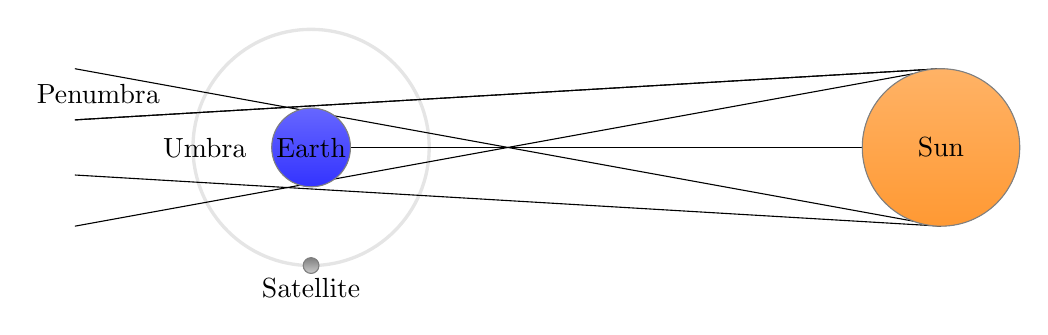
\begin{tikzpicture}
\filldraw[color=black!10, fill=white!5, very thick] (-4,0) circle (1.5);
\draw (-4,0) -- (4,0);
\draw (-7,-.35) -- (4,-1) ;
\draw (-7,-1) -- (4,1);
\draw (-7,.35) -- (4,1);
\draw (-7,.35) -- (4,1) node[midway, left= 4.3 cm] {Penumbra};;
\draw (-7,1) -- (4,-1) node[midway, left= 3.2 cm] {Umbra};
\fill[draw=black!50,top color=blue!60,bottom color=blue!80]
    (-4,0) circle (.5) node {Earth};
\fill[draw=black!50,top color=orange!60,bottom color=orange!80]
    (4,0) circle (1) node {Sun};
\fill[draw=black!50,top color=gray,bottom color=black!20]
     (-4,-1.5) circle (.1) node[below = 1pt] {Satellite};
\end{tikzpicture}
\caption{Umbra and penumbra regions from earth’s shadow}
\label{fig;uandb}
\end{figure}
The angle between the solar vector and its projection onto the orbital plane is known as the orbital beta angle $\beta$. The angle between the unit solar vector $\boldsymbol{s}$ and the unit vector normal to the orbital plane $\boldsymbol{\hat{n}}$ must be determined in order to calculate the beta angle. 
\subsection{Beta Angle Calculations}
The orbital beta angle can be calculated by the following equation
\begin{equation}
    \Phi = \beta + \frac{\pi}{2}
\end{equation}
The configuration is shown in figure \ref{fig:beta_angle} retrieved from \cite{bhatt2015thermally}.
\begin{figure}[H]
    \centering
    \includegraphics[width=0.5\textwidth]{Figures/beta_angle.png}
    \caption{Solar beta angle definition}
    \label{fig:beta_angle}
\end{figure}
The unit solar vector $\boldsymbol{s}$ and unit normal vector $\boldsymbol{\hat{n}}$ can be obtained using two Euler angle transformations. The solar vector $\boldsymbol{s}$, which points towards the sun in the celestial inertial coordinate system, is determined by two parameters, namely, Right Ascension of the Sun $\Gamma$ and Declination of the Sun $\epsilon$.

Similarly, a vector n is defined as a vector that points normal to the orbital plane and is determined by two parameters: orbital inclination $i$ and Right Ascension of Ascending Node $\Omega$. 


%\subsection{Calculations}

\section{Julian Date}
It is the time interval measured from epoch January 1, 4713 B.c., 12:00.

$J_0$ represents the Julian day number at 0 h UT (which is halfway into the Julian day). The Julian day is provided at any other UT by
\begin{equation}
    JD = J_{0}+UT
\end{equation}
Several Algorithms for calculation $J_0$ exist in literature, One of the simplest formulas is found in Boulet in \cite{boulet1991methods}.
The algorithm of calculating the JD is shown as follows
\begin{equation}
J_{0}=367 \cdot y-\operatorname{INT}\left\{\frac{7\left[y+\operatorname{INT}\left(\frac{m+9}{12}\right)\right]}{4}\right\}+\operatorname{INT}\left(\frac{275 \cdot m}{9}\right)+d+1,721,013.5    
\end{equation}
$INT(x)$ means to obtain the integer portion of x only without rounding.
Where $y$, $d$, and $m$, are numbers lying in the following ranges:
$$
\begin{gathered}
1901 \leq y \leq 2099 \\
1 \leq m \leq 12 \\
1 \leq d \leq 31
\end{gathered}
$$
The algorithm implemented in MATLAB can be found in table \ref{tab:j0}.

\begin{table}[H]
\centering
\caption{IN/OUT parameters of Julian\_day.m}
\label{tab:j0}
\begin{tabular}{lll}
\rowcolor[HTML]{000000} 
\multicolumn{3}{l}{\cellcolor[HTML]{000000}{\color[HTML]{FFFFFF} Julian\_day.m: Calculating the julian day}}                                                \\
\rowcolor[HTML]{000000} 
{\color[HTML]{FFFFFF} \textbf{IN/OUT}} & {\color[HTML]{FFFFFF} \textbf{Var. Name}} & {\color[HTML]{FFFFFF} \textbf{Description}} \\
OUT & J0 & Julian day at 0 hr UT (Universal Time)\\
IN & day & range: 1 -- 31 \\
IN & month & range: 1 -- 12\\
IN & year & range: range: 1901 to 2099
\end{tabular}%
\end{table}

\section{Sun Position Vector}
 Position vectors for the sun is needed to assess disturbance forces on satellites. When constructing a mission for sensor observation, sunrise or sunset circumstances are required. We may generate techniques for determining the local time of dawn and sunset using equations employed in coordinate reduction. This section describes useful methods for doing certain tasks \cite{vallado2001fundamentals}. 
 
 A basic approach whose findings are in the form of a MoD (mean-equator of date) vector with an accuracy of $0.01^{\degree}$ will be discussed and implemented. Because of the shortening of the expansions, it is valid from 1950 to 2050. The answer is based in part on equations that use the J2000.0 epoch \cite{vallado2001fundamentals}.
 The Algorithm can be implemented as following as proposed by \cite{vallado2001fundamentals}
 \begin{enumerate}
     \item Calculate the number of Julian centuries
     \begin{equation}
         T_{0}=\frac{J_{0}-2,451,545}{36,525}
     \end{equation}
    \item Get the value of the mean longitude of the sun
    \begin{equation}
         \lambda_{M \odot}=280.460^{\circ}+36,000 T_{0}
     \end{equation}
    \item Get the ecliptic latitude of the Sun by
    \begin{equation}
         \begin{gathered}
            \lambda_{\text {ecliptic }}=\lambda_{M \odot}+1.914666471 \sin \left(M_{\odot}\right)+0.0119994643 \sin \left(2 M_{\odot}\right) \text { where } M_{\odot}= \\
            357.291092^{\circ}+35,000.05034 T_{T D B}
        \end{gathered}
     \end{equation}
    \item Let $T_{T D B}=T_{0}$
    \item Find the position magnitude using the yielded equation
    \begin{equation}
         r_{\odot}=1.000140612-0.016708617 \cos \left(M_{\odot}\right)-0.000139589 \cos \left(2 M_{\odot}\right)
     \end{equation}
    \item Find approximate value for the obliquity of the ecliptic using
    \begin{equation}
         \varepsilon=23.439291^{\circ}-0.0130042 T_{0}
     \end{equation}
    \item The position vector in geocentric MoD is
    \begin{equation}
         \boldsymbol{r_{\odot}}=r_{\odot} \cos \left(\lambda_{\text {ecliptic }}\right) \hat{I}+r_{\odot} \cos (\varepsilon) \sin \left(\lambda_{\text {ecliptic }}\right) \hat{J}+r_{\odot} \sin (\varepsilon) \sin \left(\lambda_{\text {ecliptic }}\right) \widehat{K}
     \end{equation}
    \item The position vector in MoD is
    \begin{equation}
         \boldsymbol{r_{\odot}}=  \begin{bmatrix}
           r_{\odot} \cos \left(\lambda_{\text {ecliptic }}\right) \\
           r_{\odot} \cos (\varepsilon) \sin \left(\lambda_{\text {ecliptic }}\right)\\
           r_{\odot} \sin (\varepsilon) \sin \left(\lambda_{\text {ecliptic }}\right)
         \end{bmatrix} A U
     \end{equation}
 \end{enumerate}

The algorithm implemented in MATLAB can be found in table \ref{tab:sp}.

\begin{table}[H]
\centering
\caption{IN/OUT parameters of calc\_sun\_pos\_vector.m}
\label{tab:sp}
\begin{tabular}{lll}
\rowcolor[HTML]{000000} 
\multicolumn{3}{l}{\cellcolor[HTML]{000000}{\color[HTML]{FFFFFF} calc\_sun\_pos\_vector.m: Calculating the sun position ector}}                                                \\
\rowcolor[HTML]{000000} 
{\color[HTML]{FFFFFF} \textbf{IN/OUT}} & {\color[HTML]{FFFFFF} \textbf{Var. Name}} & {\color[HTML]{FFFFFF} \textbf{Description}} \\
OUT & r & Sun position vector\\
IN & T0 & Julian centuries \\
IN & promt & Km or AU\\
\end{tabular}%
\end{table}


\section{Sidereal Time}
A solar day is the amount of time it takes for the sun to return to its original position which comprises 24 hours. The universal time is measured by the passage of the sun through Greenwich meridian. This meridian is zero degrees terrestrial longitudinal. The sun lies on this meridian at noon UT.

A solar day is the amount of time it takes for the sun to return to its original position which comprises 24 hours. The universal time is measured by the passage of the sun through Greenwich meridian. This meridian is zero degrees terrestrial longitudinal. The sun lies on this meridian at noon UT.

The rotation of the earth relative to the fixed stars (i.e., the celestial sphere) is used to calculate sidereal time. One sidereal day is the time it takes for a distant star to return to the same location overhead to lie on the same meridian. It consists of Sidereal hours. The sidereal day is slightly shorter than the solar day due to the earth's orbit around the sun. A sidereal day has a length of 23 hours and 56 minutes. The planet spins 360 degrees in a sidereal day and 360.986 degrees in a solar day. Knowing the position of a point on the earth in relation to the geocentric equatorial frame at any given time necessitates knowing its local sidereal time. The local sidereal time of a site is calculated by first determining the Greenwich sidereal time $\theta_G$ (the Greenwich meridian's sidereal time) and then adding (or subtracting) the site's east longitude \cite{curtis2013orbital}. The concept of Julian day is used in algorithms for determining sidereal time. 

The Greenwich sidereal time $\theta_{G 0}$ at $0 h U T$ can be given as proposed by \cite{seidelmann2006explanatory} as
\begin{equation}
    \left.\theta_{G 0}=100.4606184+36,000.77004 T_{0}+0.000387933 T_{0}^{2}-2.583\left(10^{-8}\right) T_{0}^{3}\right)
\end{equation}
If the formula results in a value greater than $360^{\circ}$ or smaller than $0^{\circ}$, multiple of 360 must added or subtracted from the value to adjust it to the range.
Then, The Greenwich sidereal time $\theta_{G}$ can be calculated from by
\begin{equation}
    \theta_{G}=\theta_{G 0}+360.98564724 * \frac{U T}{24}
\end{equation}
The number of degrees an earth rotates within the day is given from
\begin{equation}
360.98564724 * \frac{U T}{24}
\end{equation}
Finally, a site's local sidereal time $\Lambda$ is computed by adding its east longitude $L$ by the Greenwich sidereal time.
\begin{equation}
\theta=\theta_{G}+\Lambda
\end{equation}



\clearpage